\documentclass{../../slides-style}

\slidetitle[Лекция 1: Об архитектуре]{Принципы разработки и проектирования ПО}{23.09.2024}

\begin{document}

    \begin{frame}[plain]
        \titlepage
    \end{frame}

    \section{Организационное}

    \begin{frame}
        \frametitle{Организационное}
        \begin{itemize}
            \item Лекционно-практический курс, две пары в неделю
            \item В конце устный экзамен и аттестация по домашним работам
            \item Материалы лекций на вики \url{https://cs-uni.ru}
            \item Балльная система
            \begin{itemize}
                \item 40\% за домашки, 60\% за экзамен
                \item Принцип мажорирующей двойки
            \end{itemize}
            \item Коммуникации --- в чате курса в Telegram, \url{https://t.me/+WqqbYo5j6dFlODAy}
            \begin{itemize}
                \item Также пишите в Telegram в личку, \url{https://t.me/yurii_litvinov}
            \end{itemize}
        \end{itemize}
    \end{frame}

    \begin{frame}
        \frametitle{Что будет в курсе}
        \begin{itemize}
            \item Объектно-ориентированное проектирование
            \item Моделирование, язык UML и, немного, другие визуальные языки
            \item Шаблоны проектирования и антипаттерны
            \item Архитектурные стили
            \item Предметно-ориентированное проектирование
            \item Проектирование распределённых приложений
            \item Развёртывание и DevOps
            \item Примеры архитектур
        \end{itemize}
    \end{frame}

    % \begin{frame}
    %     \frametitle{Критерии оценивания}
    %     \begin{itemize}
    %         \item Меньше 60\% заданий -- 0
    %         \item От 60\% до 100\% --- линейная шкала от 2 до 10 баллов
    %         \begin{itemize}
    %             \item то есть, ровно 60\% заданий --- 2 балла
    %             \item 80\% заданий --- 6 баллов
    %             \item 100\% заданий --- 10 баллов
    %         \end{itemize}
    %         \item Задачи оцениваются по 10 баллов
    %         \item В итоговой оценке практика учитывается с весом 0.4, экзамен --- 0.6
    %         \item Округление арифметическое
    %         \item ``Принцип мажорирующей двойки''
    %     \end{itemize}
    % \end{frame}

    % \begin{frame}
    %     \frametitle{Комментарии по д/з}
    %     \begin{itemize}
    %         \item Сдавать пуллреквестом в свой репозиторий и ссылку на emkn
    %         \item Будет два больших командных задания и немного мелких
    %         \item Требуется архитектурная документация
    %         \begin{itemize}
    %             \item Комментарии к каждому классу, интерфейсу и public-методу
    %             \item Краткое описание деталей реализации в README
    %         \end{itemize}
    %         \item Требуется CI и юнит-тесты
    %         \item Язык программирования --- любой
    %         \item Овердизайн и активное использование знаний с лекций приветствуются
    %         \item Некоторые требования могут показаться ненужными --- это нормально
    %         \begin{itemize}
    %             \item Мы учимся не написанию кода, а инструментам и техникам проектирования
    %         \end{itemize}
    %     \end{itemize}
    % \end{frame}

    \section{Введение}

    \begin{frame}
        \frametitle{Программа и программный продукт}
        \begin{center}
            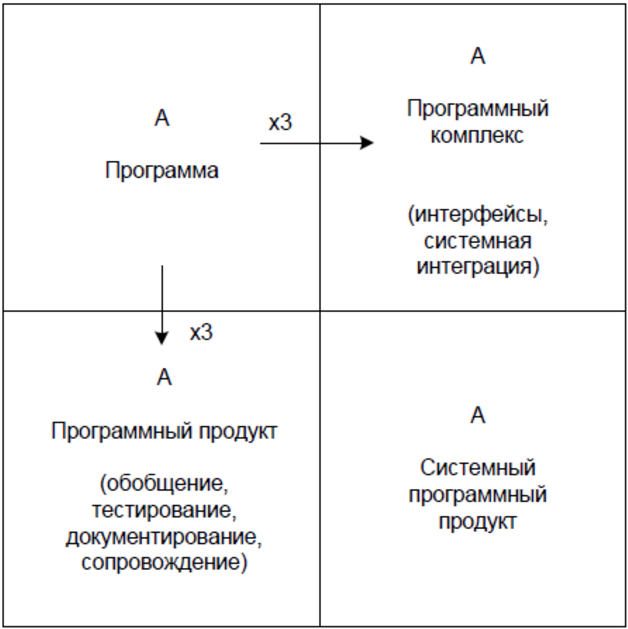
\includegraphics[width=0.5\textwidth]{brooksSquare.png}
        \end{center}
        \attribution{Ф. Брукс, <<Мифический человеко-месяц>>}
        \begin{textblock}{2}(10,-4)
            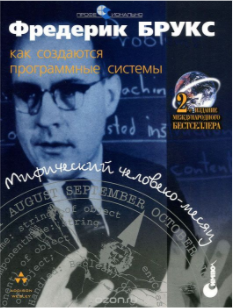
\includegraphics[width=\textwidth]{brooksCover}
        \end{textblock}
    \end{frame}

    \begin{frame}
        \frametitle{Размер типичного ПО}
        \begin{footnotesize}
            \begin{center}
                \begin{tabu} {| X[0.6 l p] | X[1 l p] |}
                    \tabucline-
                    \everyrow{\tabucline-}
                    Простая игра для iOS            & 10000 LOC  \\
                    Unix v1.0 (1971)                & 10000 LOC  \\
                    Quake 3 engine                  & 310000 LOC \\
                    Windows 3.1 (1992)              & 2.5M LOC   \\
                    Linux kernel 2.6.0 (2003)       & 5.2M LOC   \\
                    MySQL                           & 12.5M LOC  \\
                    Microsoft Office (2001)         & 25M LOC    \\
                    Microsoft Office (2013)         & 45M LOC    \\
                    Microsoft Visual Studio 2012    & 50M LOC    \\
                    Windows Vista (2007)            & 50M LOC    \\
                    Mac OS X 10.4                   & 86M LOC    \\
                \end{tabu}
            \end{center}
            \url{http://www.informationisbeautiful.net/visualizations/million-lines-of-code/}
        \end{footnotesize}
    \end{frame}

    \begin{frame}
        \frametitle{Архитектура}
        \begin{columns}
            \begin{column}{0.7\textwidth}
                \begin{itemize}
                    \item Совокупность важнейших решений об организации программной системы
                    \begin{itemize}
                        \item Эволюционирующий свод знаний
                        \item Разные точки зрения
                        \item Разный уровень детализации
                    \end{itemize}
                    \item Для чего
                    \begin{itemize}
                        \item База для реализации, <<фундамент>> системы
                        \item Инструмент для оценки трудоёмкости и отслеживания прогресса
                        \item Средство обеспечения переиспользования
                        \item Средство анализа системы ещё до того, как она реализована
                    \end{itemize}
                \end{itemize}
            \end{column}
            \begin{column}{0.3\textwidth}
                \begin{center}
                    
\includegraphics[width=\textwidth]{whatArchitecture.png}
                \end{center}
                \attribution{Интернеты}
            \end{column}
        \end{columns}
    \end{frame}

    \section{Профессия <<Архитектор>>}

    \begin{frame}
        \frametitle{Профессия <<Архитектор>>}
        \begin{itemize}
            \item Архитектор --- специально выделенный человек (или группа людей), отвечающий за:
            \begin{itemize}
                \item разработку и описание архитектуры системы
                \item доведение её до всех заинтересованных лиц
                \item контроль реализации архитектуры
                \item поддержание её актуального состояния по ходу разработки и сопровождения
            \end{itemize}
        \end{itemize}
    \end{frame}

    \begin{frame}
        \frametitle{Трудовые функции архитектора}
        \framesubtitle{По профстандарту 06.003}
        \begin{itemize}
            \item Выявление и согласование требований к программной системе с точки зрения архитектуры
            \item Выбор и моделирование архитектурного решения для реализации программной системы
            \item Разработка разделов по архитектуре проектных и эксплуатационных документов программной системы
            \item Контроль реализации и испытаний программной системы с точки зрения архитектуры
            \item Сопровождение эксплуатации программной системы с точки зрения архитектуры
        \end{itemize}
    \end{frame}

    \begin{frame}
        \frametitle{Архитектор vs разработчик}
        \begin{center}
            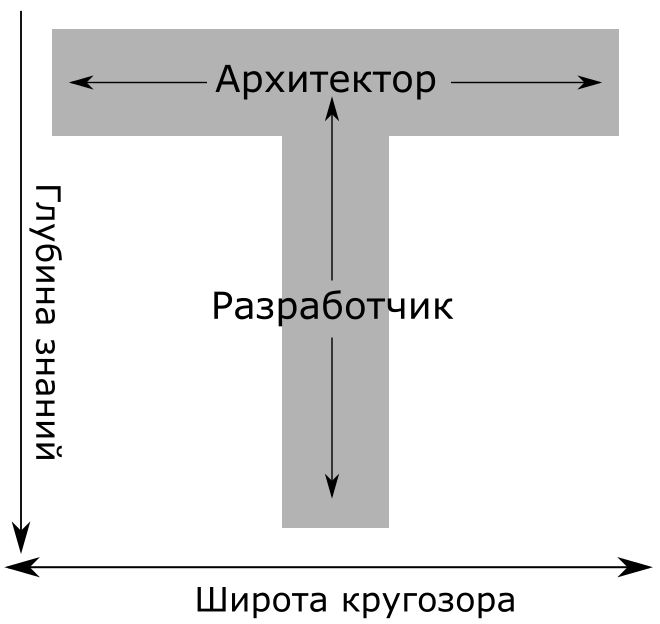
\includegraphics[width=0.35\textwidth]{architectVsDeveloper.png}
        \end{center}
        \begin{itemize}
            \item Широта знаний
            \item Коммуникационные навыки
            \item Часто архитектор играет роль разработчика и наоборот
            \begin{itemize}
                \item Архитектор в <<башне из слоновой кости>> --- это плохо
            \end{itemize}
        \end{itemize}
    \end{frame}

    \section{Пример: ПО для осциллографа}

    \begin{frame}
        \frametitle{Пример: ПО для осциллографа}
        \begin{columns}
            \begin{column}{0.6\textwidth}
                \begin{itemize}
                    \item Считывать параметры сигнала
                    \item Оцифровывать и сохранять их
                    \item Выполнять разные фильтрации и преобразования
                    \item Отображать результаты на экране
                    \begin{itemize}
                        \item С тач-скрином и встроенным хелпом
                    \end{itemize}
                    \item Возможность настройки под конкретные задачи
                \end{itemize}
            \end{column}
            \begin{column}{0.4\textwidth}
                \begin{center}
                    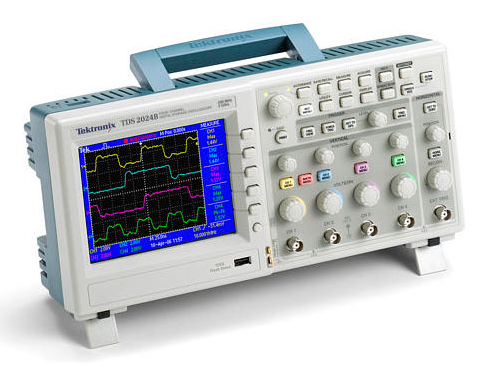
\includegraphics[width=0.9\textwidth]{oscilloscope.png}
                \end{center}
                \attribution{Hantek}
            \end{column}
        \end{columns}
        \vspace{1cm}
        \begin{tiny}
            По статье Garlan D., Shaw M. An introduction to software architecture
        \end{tiny}
    \end{frame}

    \begin{frame}
        \frametitle{Вариант 1: объектная модель}
        \begin{center}
            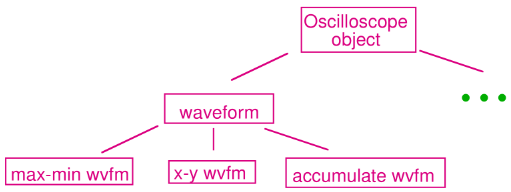
\includegraphics[width=0.5\textwidth]{oscilloscopeObjects.png}
            \attribution{Garlan D., Shaw M. An introduction to software architecture}
        \end{center}
    \end{frame}

    \begin{frame}
        \frametitle{Вариант 2: слоистая архитектура}
        \begin{center}
            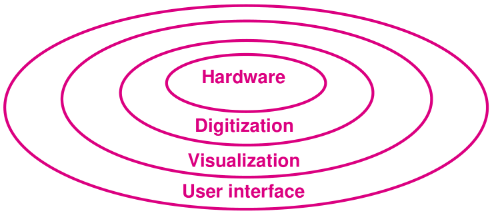
\includegraphics[width=0.5\textwidth]{oscilloscopeLayers.png}
            \attribution{Garlan D., Shaw M. An introduction to software architecture}
        \end{center}
    \end{frame}

    \begin{frame}
        \frametitle{Вариант 3: каналы и фильтры}
        \begin{center}
            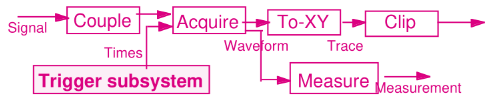
\includegraphics[width=0.5\textwidth]{oscilloscopeFilters.png}
            \attribution{Garlan D., Shaw M. An introduction to software architecture}
        \end{center}
    \end{frame}

    \begin{frame}
        \frametitle{Вариант 4: модифицированные каналы и фильтры}
        \begin{center}
            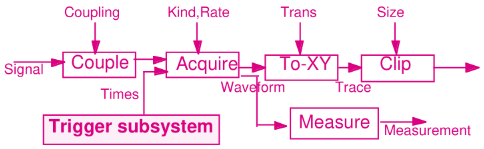
\includegraphics[width=0.5\textwidth]{oscilloscopeModifiedFilters.png}
            \attribution{Garlan D., Shaw M. An introduction to software architecture}
        \end{center}
    \end{frame}

    \begin{frame}
        \frametitle{Выводы}
        \begin{itemize}
            \item Можем делать утверждения о свойствах системы, базируясь на её структурных свойствах
            \begin{itemize}
                \item Не написав ни строчки кода и даже не выбрав язык реализации
            \end{itemize}
            \item Рассуждения очень субъективны
            \begin{itemize}
                \item Многое зависит от интуиции и вкуса архитектора, однако ошибки очень дороги
            \end{itemize}
            \item Можно выделить \emph{архитектурные стили} --- <<архитектуры архитектур>>
            \item Можно выделить \emph{архитектурные точки зрения} и \emph{архитектурные виды}
            \item Разный уровень детализации
        \end{itemize}
    \end{frame}

    \section{Архитектурные виды}

    \begin{frame}
        \frametitle{Архитектурные виды}
        \framesubtitle{Стандарт IEEE 1016-2009}
        \begin{itemize}
            \item Контекст --- фиксирует окружение системы
            \item Композиция --- описывает крупные части системы и их предназначение
            \item Логическая структура --- структура системы в терминах классов, интерфейсов и отношений между ними
            \item Зависимости --- определяет связи по данным между элементами
            \item Информационная структура --- определяет персистентные данные в системе
            \item Использование шаблонов --- документирование использования локальных паттернов проектирования
        \end{itemize}
    \end{frame}

    \begin{frame}
        \frametitle{Архитектурные виды (2)}
        \begin{itemize}
            \item Интерфейсы --- специфицирует информацию о внешних и внутренних интерфейсах
            \item Структура системы --- рекурсивное описание внутренней структуры компонентов системы
            \item Взаимодействия --- описывает взаимодействие между сущностями
            \item Динамика состояний --- описание состояний и правил переходов между состояниями
            \item Алгоритмы --- описывает в деталях поведение каждой сущности
            \item Ресурсы --- описывает использование внешних ресурсов
        \end{itemize}
    \end{frame}

    \begin{frame}
        \frametitle{Ещё про архитектурные виды}
        \begin{itemize}
            \item Пример --- \url{http://robotics.ee.uwa.edu.au/courses/design/examples/example_design.pdf}
            \item Ни один вид не обязателен
            \item Активно используются визуальные языки
            \begin{itemize}
                \item В основном как дополнение к тексту
            \end{itemize}
            \item Моделирование принципиально важно для архитектуры
            \begin{itemize}
                \item Нельзя абстрагироваться от сложности, но можно декомпозировать сложность
            \end{itemize}
        \end{itemize}
    \end{frame}

    \section{Роль архитектуры в жизненном цикле}

    \begin{frame}
        \frametitle{Роль архитектуры в жизненном цикле}
        \begin{center}
            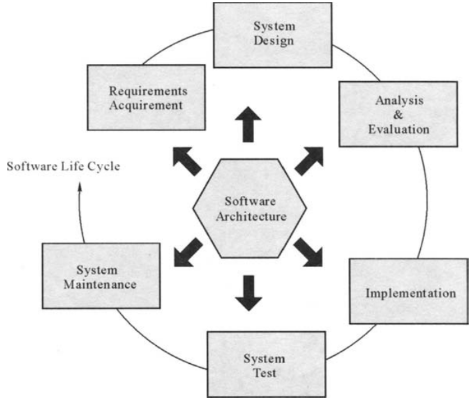
\includegraphics[width=0.5\textwidth]{architectureLifeCycle.png}
            \attribution{Z. Quin, ``Software Architecture''}
        \end{center}
    \end{frame}

    \begin{frame}
        \frametitle{Архитектура и требования}
        \begin{center}
            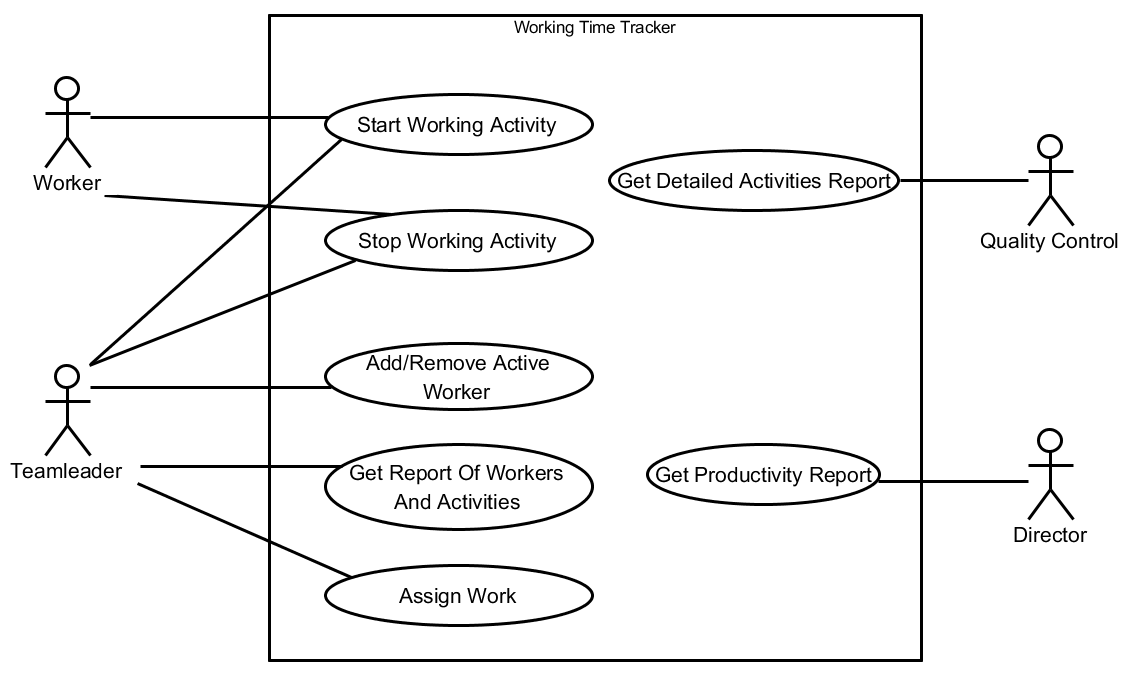
\includegraphics[width=0.8\textwidth]{useCaseDiagram.png}
        \end{center}
    \end{frame}

    \begin{frame}
        \frametitle{Требования}
        \begin{itemize}
            \item Функциональные --- то, \emph{что} система должна делать
            \item Нефункциональные --- то, \emph{как} система должна это делать
            \begin{itemize}
                \item Эффективность
                \item Масштабируемость
                \item Удобство использования
                \item Надёжность
                \item Безопасность
                \item Сопровождаемость и расширяемость
                \item ...
            \end{itemize}
            \item Ограничения
            \begin{itemize}
                \item Технические
                \item Бизнес-ограничения
            \end{itemize}
        \end{itemize}
    \end{frame}

    \begin{frame}
        \frametitle{Архитектура и проектирование}
        \begin{center}
            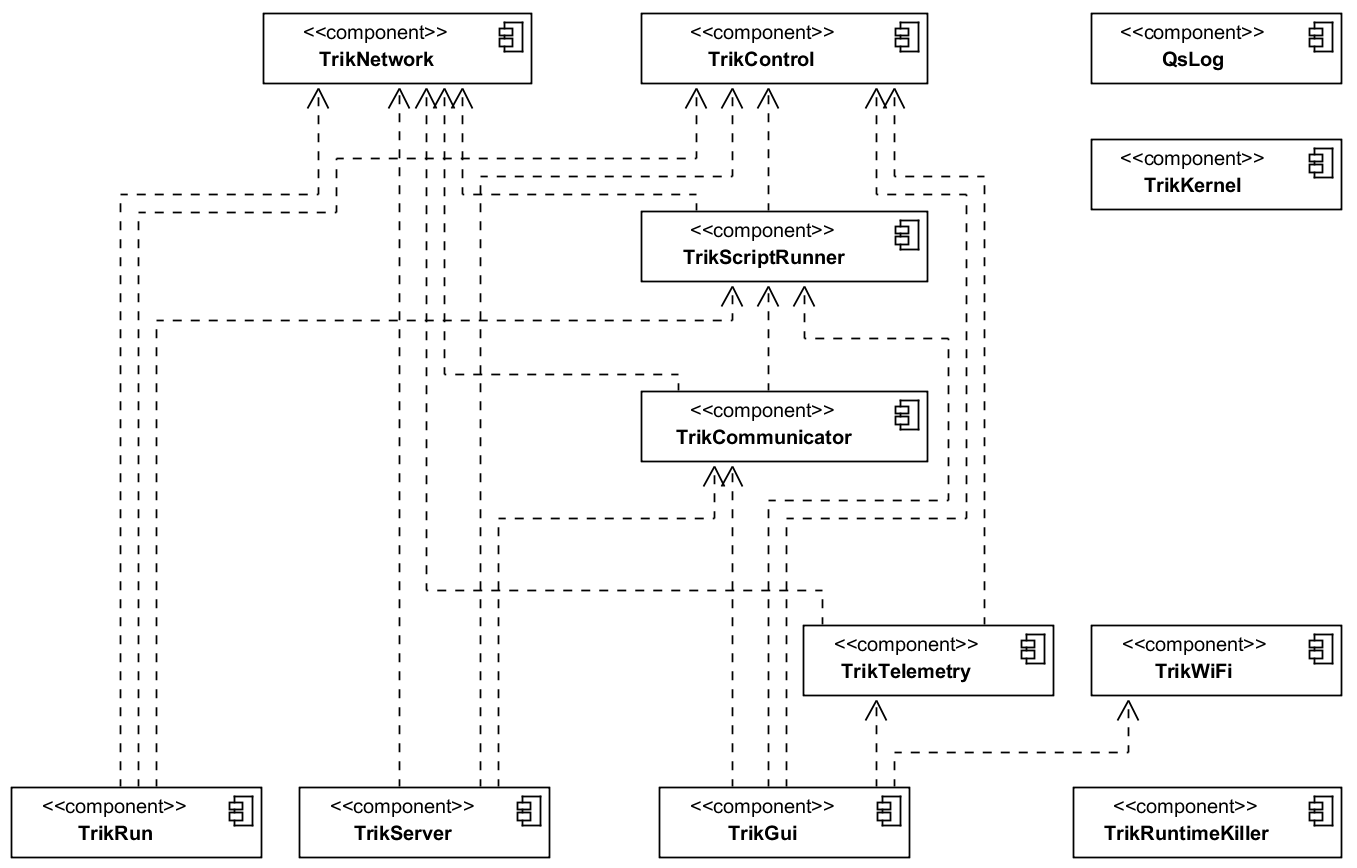
\includegraphics[width=0.8\textwidth]{trikRuntimeComponents.png}
        \end{center}
    \end{frame}

    \begin{frame}
        \frametitle{Архитектура и проектирование --- задачи}
        \begin{itemize}
            \item Декомпозиция задачи
            \item Определение границ компонентов
            \item Определение интерфейсов между компонентами
            \item Общие для всей системы вопросы
            \begin{itemize}
                \item Стратегия обработки ошибок
                \item Стратегия логирования
                \item Стратегия обновлений
                \item Стратегия разделения доступа
                \item Вопросы локализации
                \item ...
            \end{itemize}
            \item Анализ и верификация архитектуры
        \end{itemize}
    \end{frame}

    \begin{frame}
        \frametitle{Архитектура и разработка}
        \begin{itemize}
            \item \emph{prescriptive architecture} --- архитектура, как её определил архитектор
            \item \emph{descriptive architecture} --- архитектура, как она есть в системе
            \begin{itemize}
                \item Архитектура у ПО есть всегда, как вес у камня
            \end{itemize}
            \item \emph{architectural drift} --- <<сползание>> фактической архитектуры
            \begin{itemize}
                \item появление в ней важных решений, которых нет в описательной архитектуре
            \end{itemize}
            \item \emph{architectural erosion} --- <<размывание>> архитектуры
            \begin{itemize}
                \item отклонения от описательной архитектуры, нарушения ограничений
            \end{itemize}
            \item Антипаттерн <<\emph{Big ball of mud}>> --- результат эрозии
        \end{itemize}
    \end{frame}

    \section{Пример: Hadoop}

    \begin{frame}
        \frametitle{Пример: Hadoop}
        \framesubtitle{As-designed}
        \begin{center}
            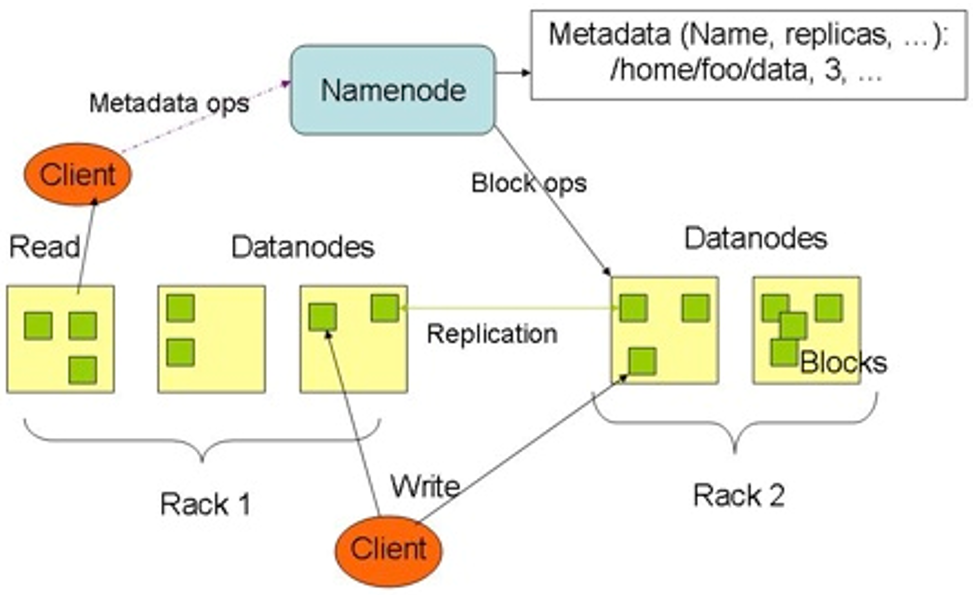
\includegraphics[width=0.6\textwidth]{hadoopPrescriptive.png}
        \end{center}
        \begin{scriptsize}\textcolor{gray}{Special thanks to prof. Nenad Medvidovic (USC) for kind permission for using his slides}\end{scriptsize}
    \end{frame}

    \begin{frame}
        \frametitle{Hadoop as-built}
        \framesubtitle{HDFS}
        \begin{center}
            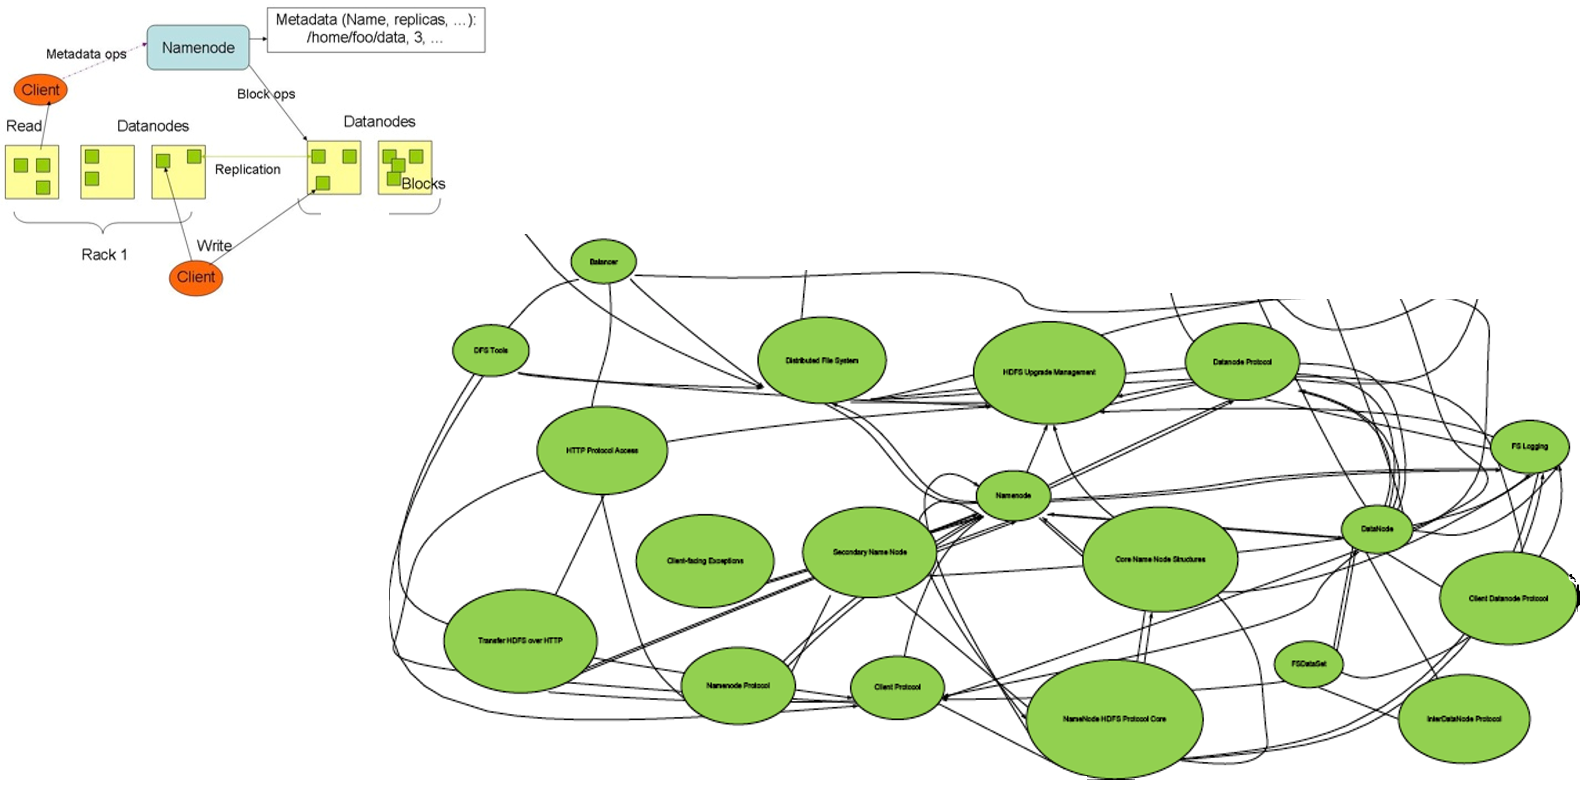
\includegraphics[width=0.9\textwidth]{hadoopDescriptive.png}
            \attribution{Nenad Medvidovic}
        \end{center}
    \end{frame}

    \begin{frame}
        \frametitle{Hadoop as-built}
        \framesubtitle{HDFS + MapReduce}
        \begin{center}
            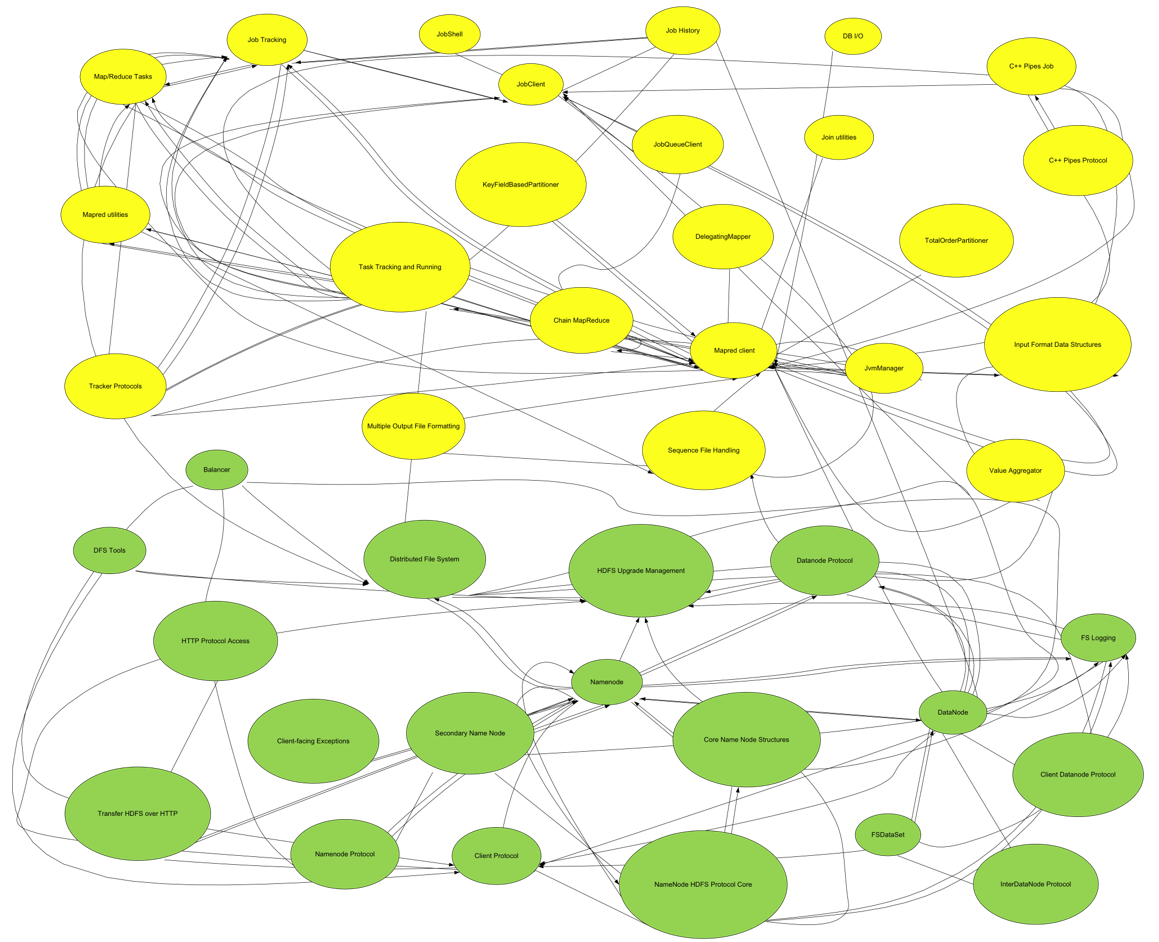
\includegraphics[width=0.7\textwidth]{hdfsMapReduce.png}
            \attribution{Nenad Medvidovic}
        \end{center}
    \end{frame}

    \begin{frame}
        \frametitle{Hadoop as-built}
        \framesubtitle{Полная архитектура}
        \begin{center}
            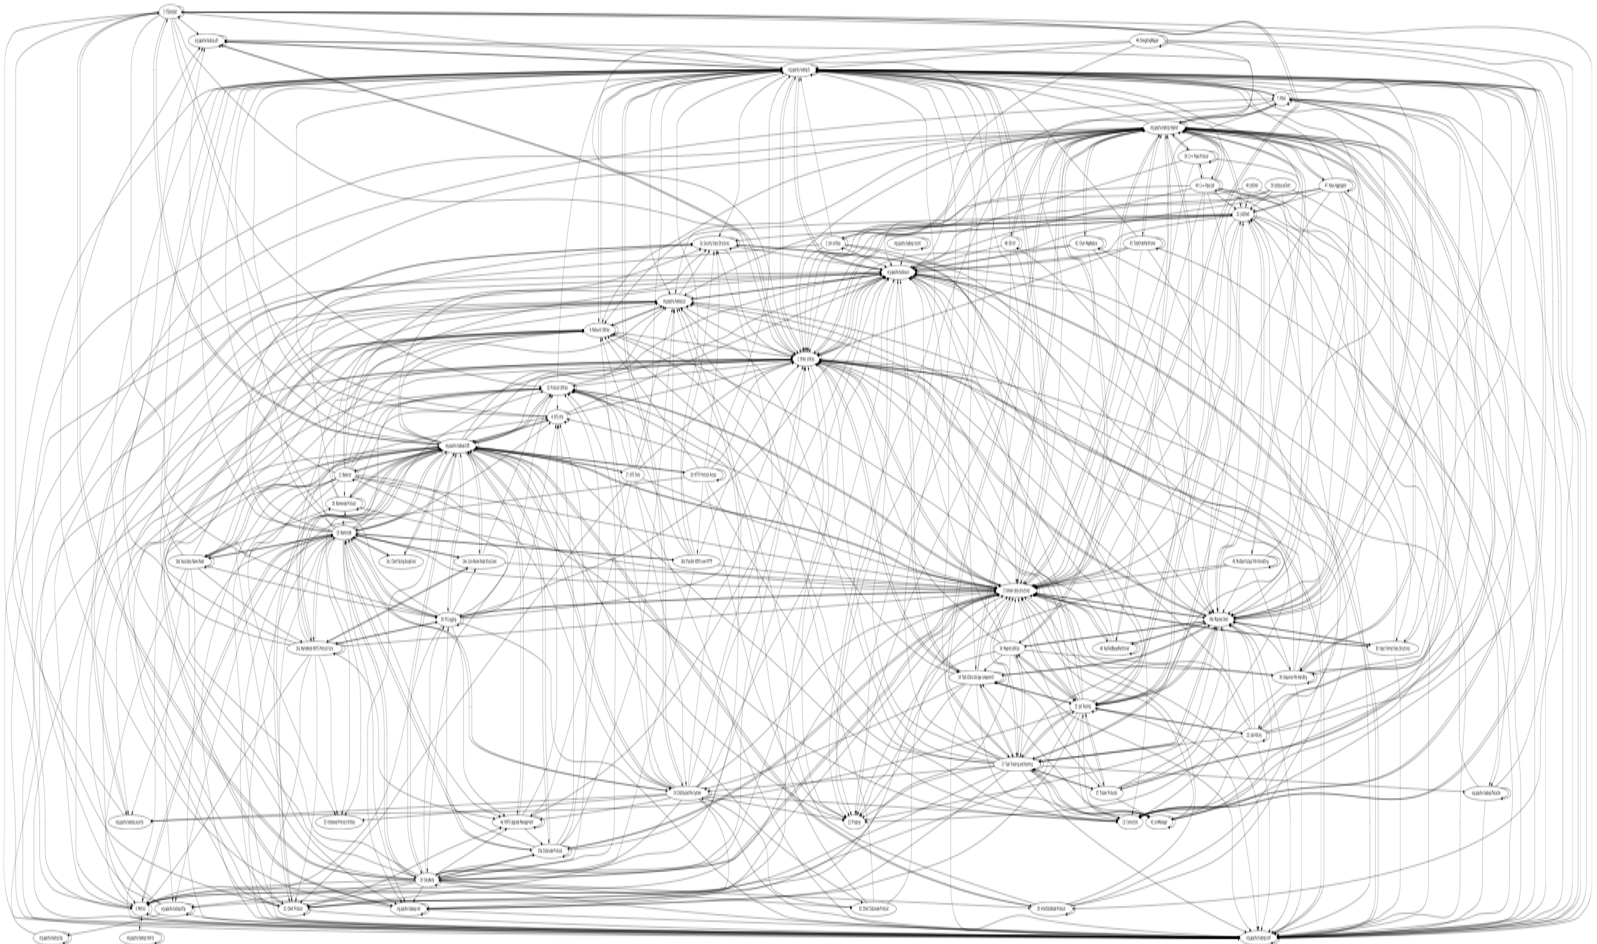
\includegraphics[width=0.9\textwidth]{hadoopFull.png}
            \attribution{Nenad Medvidovic}
        \end{center}
    \end{frame}

    \begin{frame}
        \frametitle{Hadoop as-built}
        \framesubtitle{Граф зависимостей}
        \begin{center}
            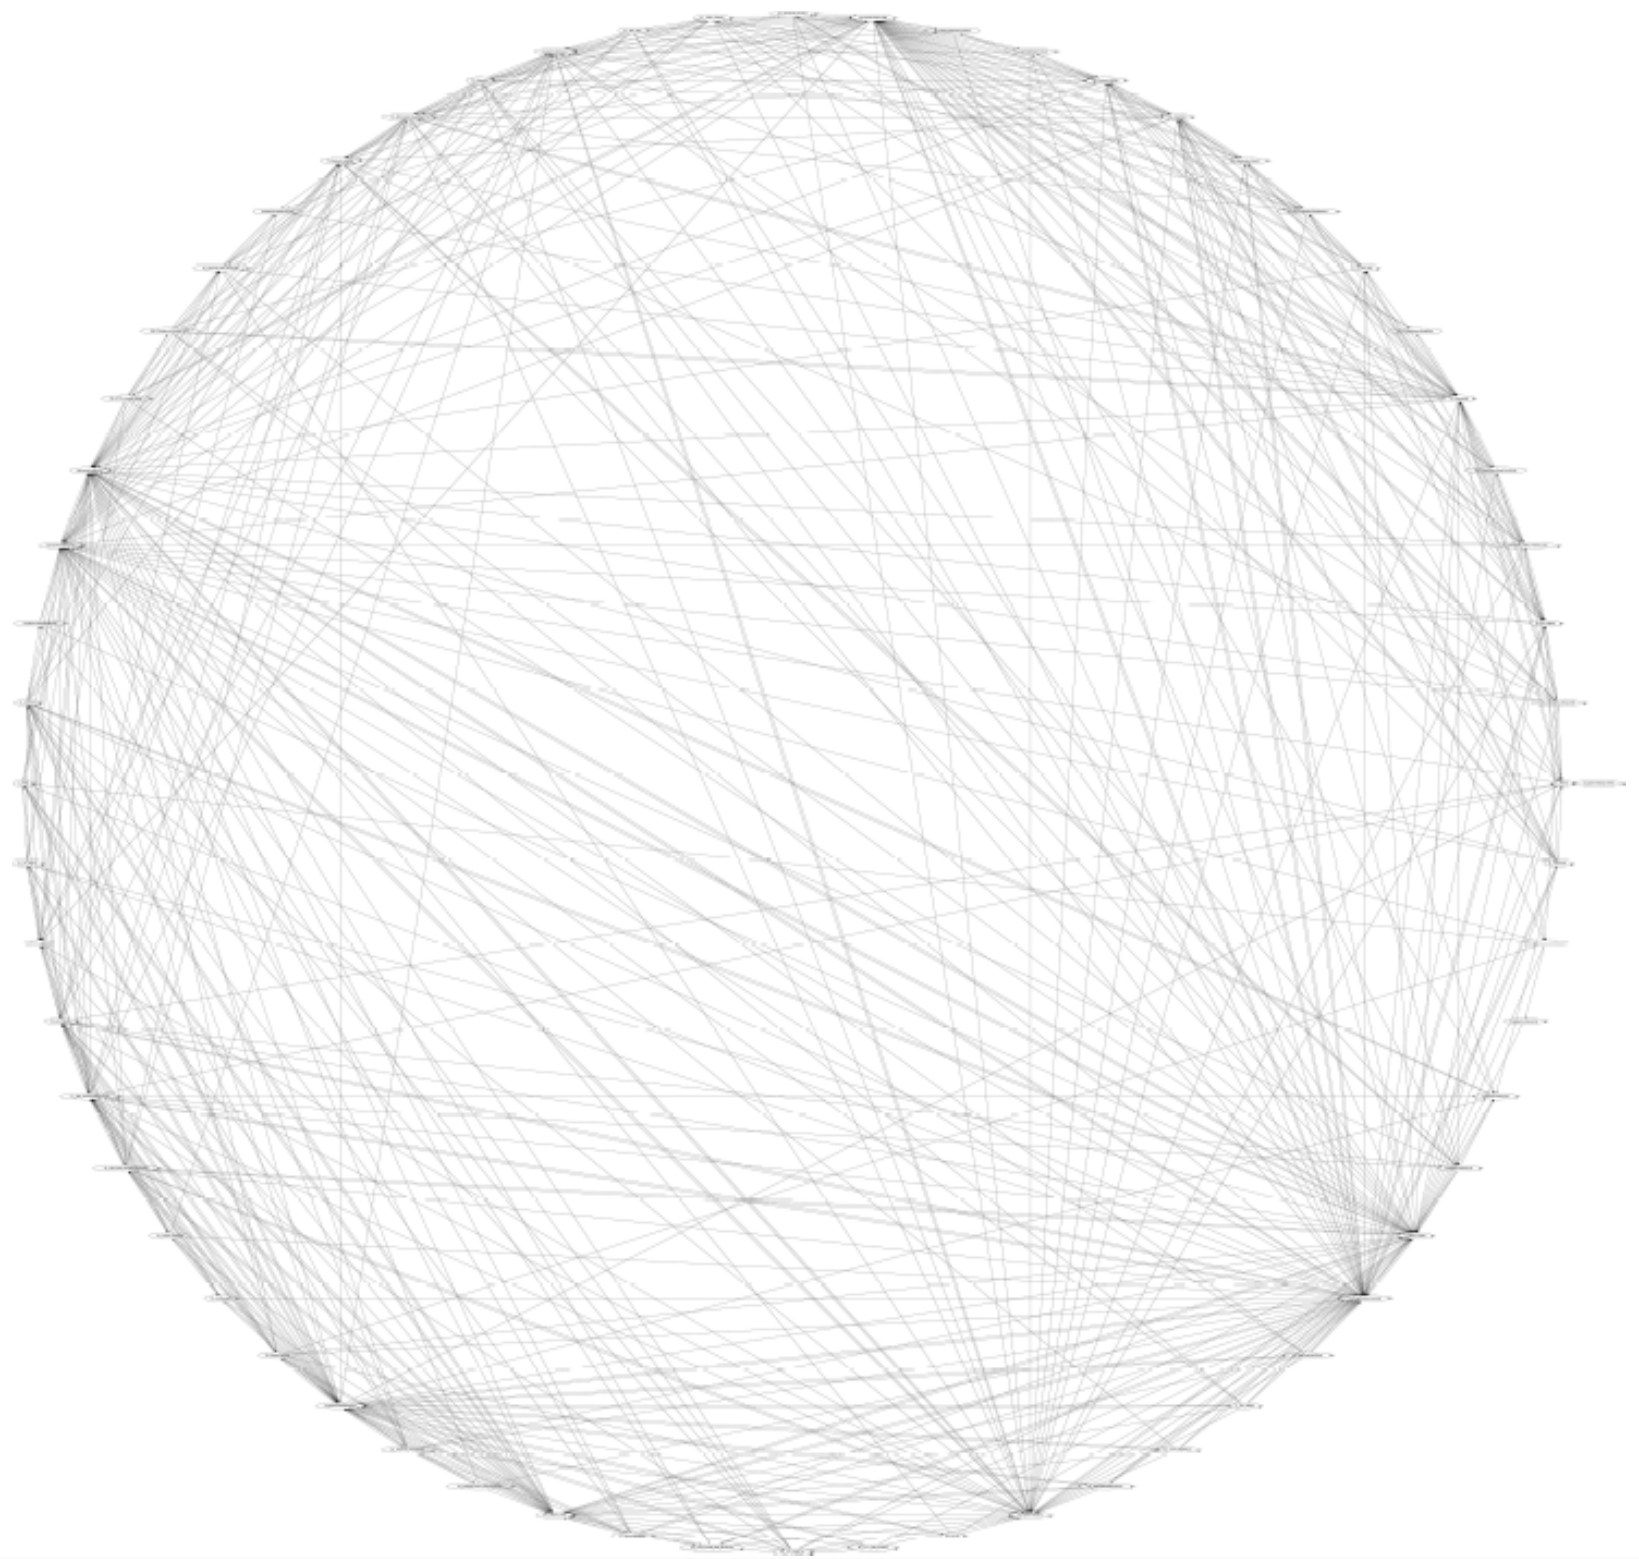
\includegraphics[width=0.5\textwidth]{hadoopDependencies.png}
            \attribution{Nenad Medvidovic}
        \end{center}
    \end{frame}

\end{document}
